\chapter{Validazione (parte 2): schemi formali}\label{ch-10}

Questa seconda parte formalizza l'uso corretto della cross-validation
per la model selection e/o la stima del rischio, con una notazione
precisa (adattata dalle slide di S. Bengio). Sono concetti semplici, ma
una notazione rigorosa evita ambiguità. Non è un ricettario: serve a
\textbf{razionalizzare} e capire in modo sistematico un approccio
rigoroso, per poi essere ragionevoli. Il tempo per eseguire gli
esperimenti dipende soprattutto dalle scelte di validazione: bisogna
evitare sia una valutazione troppo grossolana sia un processo di
valutazione infinito. In caso di dubbi, questi schemi sono comunque
meglio della fantasia.

Si parla di selezione tra configurazioni di iperparametri (indicate con
\(\theta\)), ma gli stessi schemi valgono per scegliere tra
\textbf{modelli diversi} (\(\theta\) può rappresentare anche il tipo di
modello).

\begin{boxtip}{Tenere a mente il controesempio}

Dalla parte 1: (1) le stime d'errore su TR e/o VL \textbf{non} sono
buone stime del rischio; (2) usare l'intero dataset per la selezione di
feature o modelli \textbf{pregiudica} la stima. Negli schemi che seguono
si vede esattamente dove questi errori verrebbero commessi.

\end{boxtip}

\section{Notazione}\label{notazione}

\textbf{Dati}: \(Z_1, \dots, Z_l\) è un campione casuale di una
distribuzione sconosciuta \(p(z)\), con tutti gli \(Z_i\)
\textbf{indipendenti e identicamente distribuiti} (i.i.d.).
\(D_r = \{z_1, \dots, z_r\}\) è una particolare istanza con \(r\)
elementi.

\textbf{Task}: classificazione,
\(Z = (X, Y) \in \mathbb{R}^n \times \{-1, +1\}\); regressione,
\(Z = (X, Y) \in \mathbb{R}^n \times \mathbb{R}\).

\textbf{Loss} (``interna''): classificazione \(L((x,y), h) = 0\) se
\(h(x) = y\), \(1\) altrimenti; regressione
\(L((x,y), h) = (h(x) - y)^2\).

\textbf{Obiettivo}: minimizzare il \textbf{rischio atteso} (errore vero)
su \(H\): \[
R(h) = \mathbb{E}_Z[L(z, h)] = \int_Z L(z, h)\,p(z)\,dz, \qquad h^* = \arg\min_{h \in H} R(h).
\] Il problema: \(p(z)\) è sconosciuta e non abbiamo accesso a tutti gli
\(L(z,h)\).

\textbf{Rischio empirico} su un insieme finito \(D_r\): \[
R_{emp}(h, D_r) = \frac{1}{r}\sum_{i=1}^{r} L(z_i, h).
\]

\begin{boxwarning}{Uso generale di \(R_{emp}\)}

Qui \(R_{emp}\) è inteso in senso generale, come \textbf{surrogato di
\(R\)} su un insieme finito di dati, usato per il training, la model
selection o l'assessment a seconda della partizione. Da non confondere
con il \(R_{emp}\) della SLT, che è specificamente l'errore di training:
in questa notazione è \(R_{emp}(h, D_{TR})\).

\end{boxwarning}

\section{Metodologia: identificare
l'obiettivo}\label{metodologia-identificare-lobiettivo}

\begin{enumerate}
\def\labelenumi{\arabic{enumi}.}
\tightlist
\item
  Dare il \textbf{miglior modello} ottenibile da un dataset? → serve la
  \textbf{model selection}.
\item
  Dare le \textbf{prestazioni attese} di un modello ottenuto per
  minimizzazione del rischio empirico? → serve la \textbf{model
  assessment} (stima del rischio).
\item
  Dare \textbf{entrambi}? → servono tutte e due.
\end{enumerate}

Il dataset originale \(D_l\) verrà usato per questi diversi scopi.

\section{Model selection}\label{model-selection}

\subsection{Hold-out}\label{hold-out}

\begin{boxabstract}{Model selection con hold-out}

\begin{itemize}
\tightlist
\item
  Scegliere uno spazio delle ipotesi con iperparametro \(\theta\).
\item
  Dividere \(D_l\) in \(D_{TR} = \{z_1, \dots, z_{tr}\}\) e
  \(D_{VL} = \{z_{tr+1}, \dots, z_{tr+vl}\}\), con \(tr + vl = l\).
\item
  Per ogni valore \(\theta_m\) {[}\textbf{grid search}{]}:

  \begin{itemize}
  \tightlist
  \item
    \(h^*_{\theta_m}(D_{TR}) = \arg\min_{h \in H_{\theta_m}} R_{emp}(h, D_{TR})\)
    {[}\textbf{training}{]};
  \item
    stimare \(R(h^*_{\theta_m})\) con
    \(R_{emp}(h^*_{\theta_m}, D_{VL}) = \frac{1}{vl}\sum_{z_i \in D_{VL}} L(z_i, h^*_{\theta_m}(D_{TR}))\).
  \end{itemize}
\item
  Scegliere \(\theta^*_m = \arg\min_{\theta_m} R(h^*_{\theta_m})\)
  {[}miglior risultato sul VL{]}.
\item
  Restituire
  \(h^*(D_l) = \arg\min_{h \in H_{\theta^*_m}} R_{emp}(h, D_l)\)
  {[}\textbf{riaddestramento} su tutti gli \(l\) dati{]}.
\end{itemize}

\end{boxabstract}

La stima di \(R\) sul VL serve \textbf{solo} alla model selection e
\textbf{non viene restituita} come stima del rischio: restituirla
sarebbe esattamente l'errore (1) del controesempio.

\subsection{K-fold cross-validation}\label{k-fold-cross-validation}

\begin{boxabstract}{Model selection con K-fold CV}

\begin{itemize}
\tightlist
\item
  Scegliere uno spazio delle ipotesi con iperparametro \(\theta\).
\item
  Dividere \(D_l\) in \(K\) parti distinte e uguali \(D_1, \dots, D_K\);
  sia \(\bar D_k\) il complementare di \(D_k\).
\item
  Per ogni valore \(\theta_m\) {[}\textbf{grid search}{]}:

  \begin{itemize}
  \tightlist
  \item
    per ogni parte \(D_k\) {[}\textbf{ciclo sui fold}{]}:

    \begin{itemize}
    \tightlist
    \item
      \(h^*_{\theta_m}(\bar D_k) = \arg\min_{h \in H_{\theta_m}} R_{emp}(h, \bar D_k)\)
      {[}training{]};
    \item
      stimare \(R(h^*_{\theta_m}(\bar D_k))\) con
      \(R_{emp}(h^*_{\theta_m}(\bar D_k), D_k) = \frac{1}{|D_k|}\sum_{z_i \in D_k} L(z_i, h^*_{\theta_m}(\bar D_k))\);
    \end{itemize}
  \item
    stimare \(R(h^*_{\theta_m}(D_l))\) con la media
    \(\frac{1}{K}\sum_k R(h^*_{\theta_m}(\bar D_k))\).
  \end{itemize}
\item
  Scegliere \(\theta^*_m = \arg\min_{\theta_m} R(h^*_{\theta_m}(D_l))\)
  {[}migliore su tutte le CV{]}.
\item
  Restituire
  \(h^*(D_l) = \arg\min_{h \in H_{\theta^*_m}} R_{emp}(h, D_l)\)
  {[}riaddestramento{]}.
\end{itemize}

\end{boxabstract}

\begin{figure}[htbp]
\centering
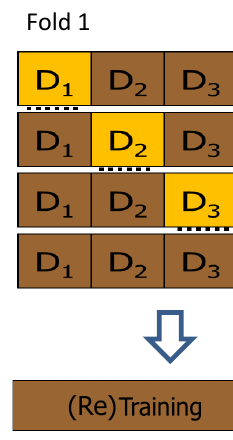
\includegraphics[width=0.31\linewidth,height=0.42\textheight,keepaspectratio]{images/10-val2_kfold-selezione.png}
\caption{K-fold CV per la model selection, seguita dal riaddestramento.}
\end{figure}

\begin{boxwarning}{Attenzione all'ordine}

Ogni iterazione \textbf{riparte da zero}, con addestramento e stima
locali alla suddivisione. Se ad esempio si usasse un modello addestrato
nello split 1 per valutare lo split 2, si userebbe come validazione
dello split 2 una parte (\(D_2\)) che era stata usata per addestrare
nello split 1.

\end{boxwarning}

\section{Stima del rischio (model
assessment)}\label{stima-del-rischio-model-assessment}

\subsection{Hold-out}\label{hold-out-1}

\begin{boxabstract}{Model assessment con hold-out}

\begin{itemize}
\tightlist
\item
  Dividere \(D_l\) in \(D_{TR}\) e \(D_{TS}\), con \(tr + ts = l\).
  \textbf{Il test set va separato ADESSO} (non dopo): altrimenti si
  commette l'errore (2) del controesempio.
\item
  \(h^*(D_{TR}) = \arg\min_{h \in H} R_{emp}(h, D_{TR})\) {[}training;
  può includere una model selection interna su \(D_{TR}\){]}.
\item
  Stimare \(R(h^*(D_{TR}))\) con
  \(R_{emp}(h^*(D_{TR}), D_{TS}) = \frac{1}{ts}\sum_{z_i \in D_{TS}} L(z_i, h^*(D_{TR}))\)
  {[}\textbf{errore di test}{]}.
\end{itemize}

\end{boxabstract}

\subsection{K-fold cross-validation}\label{k-fold-cross-validation-1}

\begin{boxabstract}{Model assessment con K-fold CV}

\begin{itemize}
\tightlist
\item
  Dividere \(D_l\) in \(K\) parti distinte e uguali.
\item
  Per ogni parte \(D_k\) {[}ciclo sui fold{]}:

  \begin{itemize}
  \tightlist
  \item
    \(h^*(\bar D_k) = \arg\min_{h \in H} R_{emp}(h, \bar D_k)\)
    {[}training; può includere una model selection{]};
  \item
    stimare \(R(h^*(\bar D_k))\) con \(R_{emp}(h^*(\bar D_k), D_k)\)
    {[}errore di test di ogni iterazione{]}.
  \end{itemize}
\item
  Stimare \(R(h^*(D_l))\) con la media
  \(\frac{1}{K}\sum_k R(h^*(\bar D_k))\).
\end{itemize}

\end{boxabstract}

Con \(K = l\) si ha la \textbf{leave-one-out CV}. Non si violano i
principi: i risultati di test non vengono mai usati per addestrare o
selezionare, in nessuna iterazione.

\section{Combinare model selection e model
assessment}\label{combinare-model-selection-e-model-assessment}

Quando si vogliono sia il modello migliore sia il suo rischio atteso,
bisogna combinare i metodi. Ad esempio:

\begin{itemize}
\tightlist
\item
  \textbf{hold-out} con training--validation--test (servono tre insiemi
  separati);
\item
  \textbf{K-fold CV + test}: cross-validation sul training set, poi test
  su un insieme separato;
\item
  \textbf{K-fold CV esterna per il test}, con hold-out interno per la
  model selection;
\item
  \textbf{double (nested) cross-validation}: per ogni fold esterno, una
  cross-validation annidata sugli altri \(K-1\).
\end{itemize}

Altri aspetti: considerare le \textbf{diverse prove} (inizializzazioni
diverse di una rete) nel calcolo delle medie su TR, VL, TS. Più in
generale: confrontare i risultati con altri metodi, usare \textbf{test
statistici} per verificarne la significatività, verificare il modello su
più dataset.

\subsection{Hold-out
training--validation--test}\label{hold-out-trainingvalidationtest}

\begin{boxabstract}{Schema TR--VL--TS}

\begin{itemize}
\tightlist
\item
  Dividere \(D_l\) in \(D_{TR}\), \(D_{VL}\), \(D_{TS}\).
\item
  Per ogni \(\theta_m\): addestrare \(h^*_{\theta_m}(D_{TR})\) e
  calcolare \(R_{emp}(h^*_{\theta_m}(D_{TR}), D_{VL})\).
\item
  Scegliere \(\theta^*_m\) con il miglior risultato sul VL.
\item
  Riaddestrare \(h^*(D_{TR} \cup D_{VL})\) con \(\theta^*_m\).
\item
  Stimare \(R\) con
  \(\frac{1}{ts}\sum_{z_i \in D_{TS}} L(z_i, h^*(D_{TR} \cup D_{VL}))\).
\end{itemize}

\end{boxabstract}

Il riaddestramento può usare una parte dei dati come VL per l'early
stopping.

\begin{boxquestion}{Si può riaddestrare ancora su tutto \(D_l\)?}

Il riaddestramento finale su tutti i dati (TR+VL+TS) \textbf{non usa} i
risultati del test per alcuna scelta: il modello finale avrà in generale
prestazioni pari o migliori della stima (più dati), che resta valida
come stima (leggermente pessimistica) del rischio della procedura.
L'importante è che il test non abbia influenzato nessuna decisione.

\end{boxquestion}

\subsection{K-fold CV per la selezione + hold-out per il
test}\label{k-fold-cv-per-la-selezione-hold-out-per-il-test}

\begin{boxabstract}{Schema CV + test}

\begin{itemize}
\tightlist
\item
  Dividere \(D_l\) in \(D_{TR}\) (il \emph{design set}) e \(D_{TS}\).
\item
  Per ogni \(\theta_m\): stimare \(R(h^*_{\theta_m}(D_{TR}))\) con una
  K-fold CV su \(D_{TR}\) (errore di validazione medio sui fold).
\item
  Scegliere \(\theta^*_m\) con la migliore stima.
\item
  Riaddestrare \(h^*(D_{TR})\).
\item
  Stimare \(R\) con l'errore su \(D_{TS}\).
\end{itemize}

\end{boxabstract}

\subsection{K-fold CV per il test con hold-out interno per la
selezione}\label{k-fold-cv-per-il-test-con-hold-out-interno-per-la-selezione}

In ogni riga della K-fold esterna, un fold fa da test e il resto viene
diviso (arbitrariamente e con shuffling) in TR e VL per la model
selection. La descrizione in meta-algoritmo è lasciata per esercizio.

\begin{figure}[htbp]
\centering
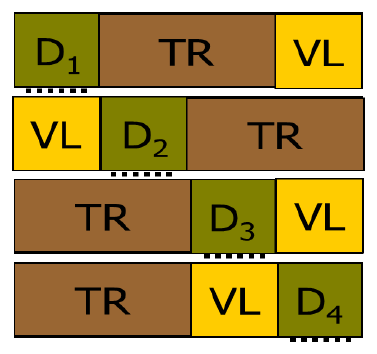
\includegraphics[width=0.31\linewidth,height=0.42\textheight,keepaspectratio]{images/10-val2_kfold-holdout.png}
\caption{K-fold CV esterna per il test, con hold-out TR/VL interno per la model
selection (il riaddestramento non è mostrato).}
\end{figure}

\begin{boxnote}{Nessun modello unico}

Questo processo \textbf{non fornisce un modello finale}: dà solo una
stima del rischio della \textbf{classe} di modelli considerata, perché
potenzialmente ogni riga seleziona un modello diverso.

\end{boxnote}

\subsection{Double (nested) K-fold CV}\label{double-nested-k-fold-cv}

\begin{boxabstract}{Double K-fold CV}

\begin{itemize}
\tightlist
\item
  Dividere \(D_l\) in \(K\) parti distinte e uguali.
\item
  Per ogni parte \(D_k\) {[}\textbf{ciclo esterno}{]}:

  \begin{itemize}
  \tightlist
  \item
    scegliere \(h^*(\bar D_k)\) con una \textbf{K-fold CV interna} su
    \(\bar D_k\) (con \(K'\) eventualmente diverso da \(K\))
    {[}\textbf{ciclo interno}{]};
  \item
    stimare \(R(h^*(\bar D_k))\) con \(R_{emp}(h^*(\bar D_k), D_k)\)
    {[}errore di test per ogni split esterno{]}.
  \end{itemize}
\item
  Stimare \(R(h^*(D_l))\) con la media sui fold di test.
\end{itemize}

\end{boxabstract}

\begin{figure}[htbp]
\centering
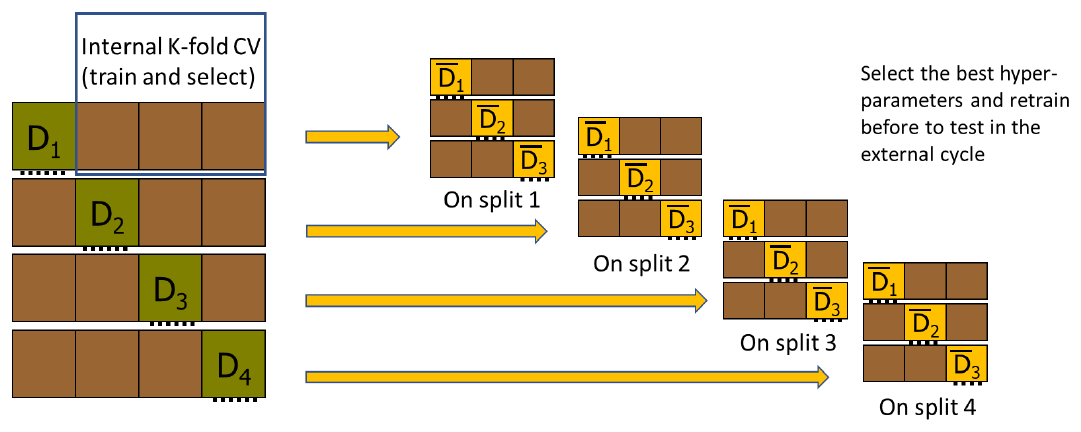
\includegraphics[width=0.89\linewidth,height=0.42\textheight,keepaspectratio]{images/10-val2_double-cv.png}
\caption{Double K-fold CV: in ogni split esterno una CV interna seleziona gli
iperparametri.}
\end{figure}

Anche qui \textbf{non si ottiene un modello finale unico}, perché ogni
ciclo esterno può scegliere iperparametri diversi: si ottiene una stima
del rischio della classe di modelli/algoritmo, con anche la sua
\textbf{varianza} (deviazione standard sui fold). Se serve un modello
finale unico si esegue una \textbf{model selection separata} (hold-out o
K-fold CV) e un eventuale riaddestramento finale.

Questo non viola le regole: l'errore di test è già stato stimato e i
risultati di test non vengono mai usati per la selezione; il modello
finale avrà un errore atteso nell'intervallo stimato. Per questo non è
semplicemente vero che ``il test viene sempre per ultimo'': qui avviene
\textbf{prima} dell'ultima model selection (anche se può sembrare
anti-intuitivo).

La double CV sfrutta meglio \textbf{tutti} i dati per addestramento e
valutazione (sia per la selezione sia per la valutazione), al prezzo di
un costo computazionale elevato.

\begin{figure}[htbp]
\centering
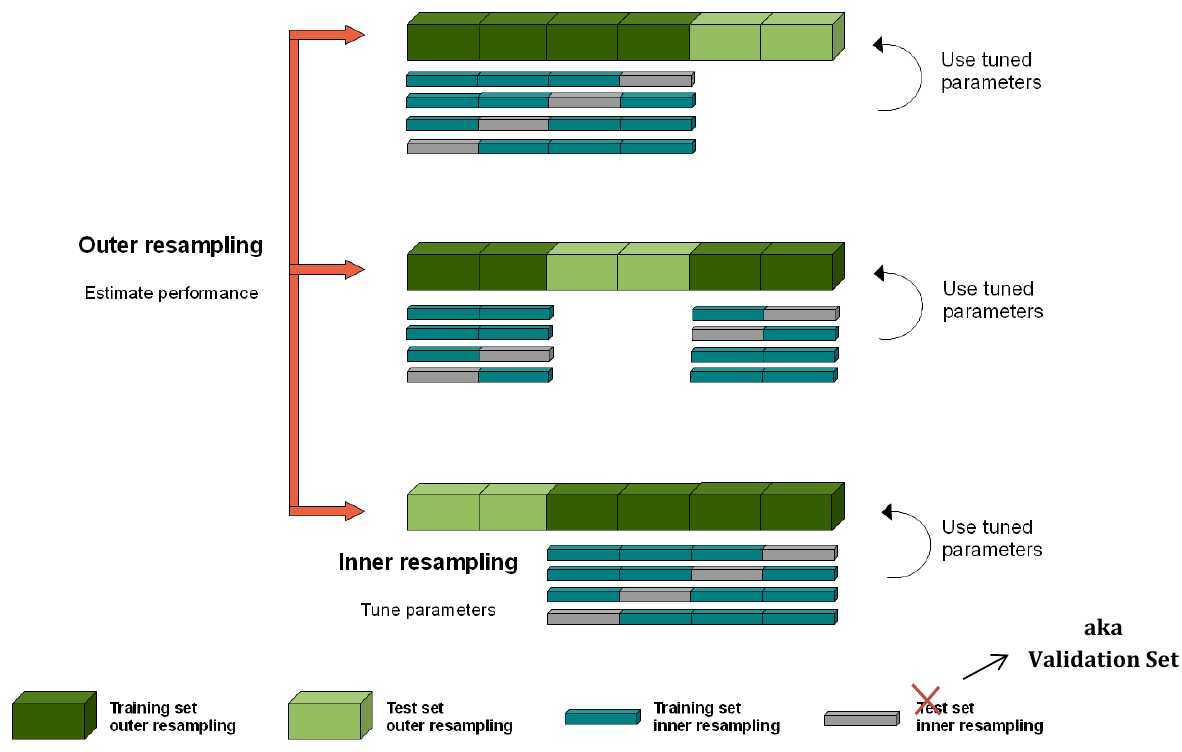
\includegraphics[width=0.80\linewidth,height=0.42\textheight,keepaspectratio]{images/10-val2_double-cv-2.png}
\caption{Un'altra vista della double CV: resampling esterno per stimare le
prestazioni, interno per regolare i parametri.}
\end{figure}

\begin{figure}[htbp]
\centering
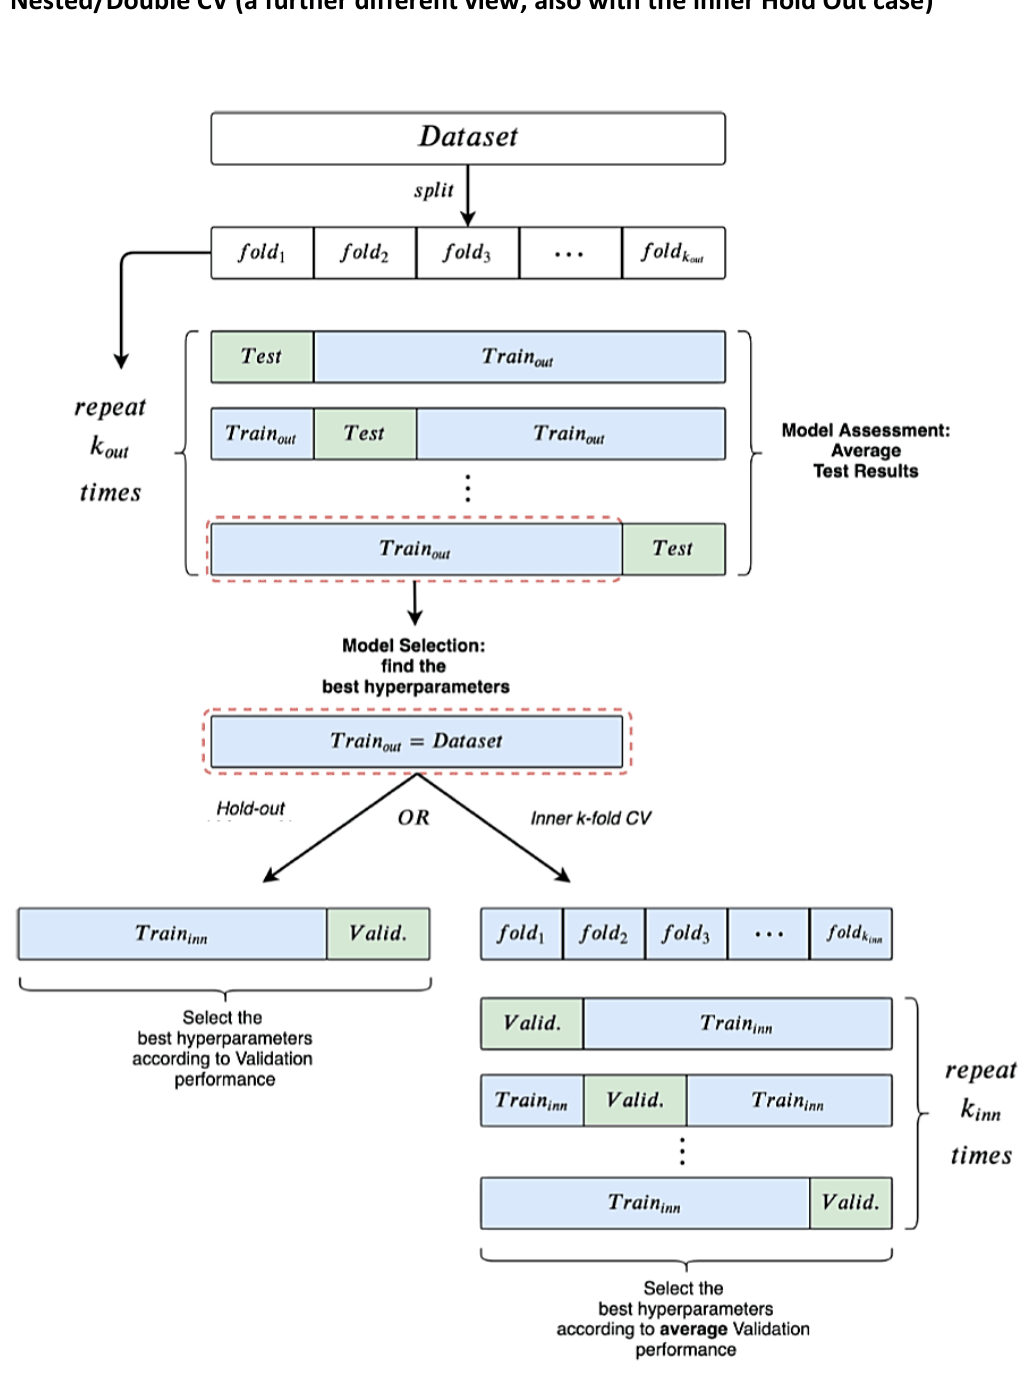
\includegraphics[width=0.63\linewidth,height=0.42\textheight,keepaspectratio]{images/10-val2_nested-cv.png}
\caption{Nested CV, anche nella variante con hold-out interno.}
\end{figure}

\begin{boxabstract}{Sintesi}

Prima si identifica l'obiettivo (modello migliore, stima delle
prestazioni, o entrambi), poi si sceglie lo schema. In tutti gli schemi
corretti: il \textbf{test è separato prima} di ogni scelta, le stime sul
\textbf{VL non vengono restituite} come stime del rischio, ogni
iterazione di CV \textbf{riparte da zero}. Gli schemi combinati più
usati sono TR--VL--TS, CV+test e la double CV.

\end{boxabstract}

\begin{boxquestion}{Possibili domande d'esame}

\begin{itemize}
\tightlist
\item
  Scrivere l'algoritmo di model selection con K-fold CV.
\item
  Scrivere l'algoritmo di model assessment con K-fold CV.
\item
  Descrivere la double (nested) CV. Restituisce un modello?
\item
  Collegare gli errori (1) e (2) del controesempio agli schemi formali.
\end{itemize}

\end{boxquestion}
